% This is "sig-alternate.tex" V2.1 April 2013
% This file should be compiled with V2.5 of "sig-alternate.cls" May 2012
%
% This example file demonstrates the use of the 'sig-alternate.cls'
% V2.5 LaTeX2e document class file. It is for those submitting
% articles to ACM Conference Proceedings WHO DO NOT WISH TO
% STRICTLY ADHERE TO THE SIGS (PUBS-BOARD-ENDORSED) STYLE.
% The 'sig-alternate.cls' file will produce a similar-looking,
% albeit, 'tighter' paper resulting in, invariably, fewer pages.
%
% ----------------------------------------------------------------------------------------------------------------
% This .tex file (and associated .cls V2.5) produces:
%       1) The Permission Statement
%       2) The Conference (location) Info information
%       3) The Copyright Line with ACM data
%       4) NO page numbers
%
% as against the acm_proc_article-sp.cls file which
% DOES NOT produce 1) thru' 3) above.
%
% Using 'sig-alternate.cls' you have control, however, from within
% the source .tex file, over both the CopyrightYear
% (defaulted to 200X) and the ACM Copyright Data
% (defaulted to X-XXXXX-XX-X/XX/XX).
% e.g.
% \CopyrightYear{2007} will cause 2007 to appear in the copyright line.
% \crdata{0-12345-67-8/90/12} will cause 0-12345-67-8/90/12 to appear in the copyright line.
%
% ---------------------------------------------------------------------------------------------------------------
% This .tex source is an example which *does* use
% the .bib file (from which the .bbl file % is produced).
% REMEMBER HOWEVER: After having produced the .bbl file,
% and prior to final submission, you *NEED* to 'insert'
% your .bbl file into your source .tex file so as to provide
% ONE 'self-contained' source file.
%
% ================= IF YOU HAVE QUESTIONS =======================
% Questions regarding the SIGS styles, SIGS policies and
% procedures, Conferences etc. should be sent to
% Adrienne Griscti (griscti@acm.org)
%
% Technical questions _only_ to
% Gerald Murray (murray@hq.acm.org)
% ===============================================================
%
% For tracking purposes - this is V2.0 - May 2012

\documentclass{sig-alternate-05-2015}
\usepackage{listings}
\usepackage{float}

\begin{document}

% Copyright
%\setcopyright{acmcopyright}
%\setcopyright{acmlicensed}
%\setcopyright{rightsretained}
%\setcopyright{usgov}
%\setcopyright{usgovmixed}
%\setcopyright{cagov}
%\setcopyright{cagovmixed}

%Conference
%\conferenceinfo{PLDI '13}{June 16--19, 2013, Seattle, WA, USA}

%\acmPrice{\$15.00}

%
% --- Author Metadata here ---
%\conferenceinfo{WOODSTOCK}{'97 El Paso, Texas USA}
%\CopyrightYear{2007} % Allows default copyright year (20XX) to be over-ridden - IF NEED BE.
%\crdata{0-12345-67-8/90/01}  % Allows default copyright data (0-89791-88-6/97/05) to be over-ridden - IF NEED BE.
% --- End of Author Metadata ---

\title{Report for Homework 1}
\subtitle{CS 7930 Social Media Mining\\
Spring 2016}
%\subtitle{[Extended Abstract]
%\titlenote{A full version of this paper is available as
%\textit{Author's Guide to Preparing ACM SIG Proceedings Using
%\LaTeX$2_\epsilon$\ and BibTeX} at
%\texttt{www.acm.org/eaddress.htm}}}
%
% You need the command \numberofauthors to handle the 'placement
% and alignment' of the authors beneath the title.
%
% For aesthetic reasons, we recommend 'three authors at a time'
% i.e. three 'name/affiliation blocks' be placed beneath the title.
%
% NOTE: You are NOT restricted in how many 'rows' of
% "name/affiliations" may appear. We just ask that you restrict
% the number of 'columns' to three.
%
% Because of the available 'opening page real-estate'
% we ask you to refrain from putting more than six authors
% (two rows with three columns) beneath the article title.
% More than six makes the first-page appear very cluttered indeed.
%
% Use the \alignauthor commands to handle the names
% and affiliations for an 'aesthetic maximum' of six authors.
% Add names, affiliations, addresses for
% the seventh etc. author(s) as the argument for the
% \additionalauthors command.
% These 'additional authors' will be output/set for you
% without further effort on your part as the last section in
% the body of your article BEFORE References or any Appendices.

\numberofauthors{1} %  in this sample file, there are a *total*
% of EIGHT authors. SIX appear on the 'first-page' (for formatting
% reasons) and the remaining two appear in the \additionalauthors section.
%
\author{
% You can go ahead and credit any number of authors here,
% e.g. one 'row of three' or two rows (consisting of one row of three
% and a second row of one, two or three).
%
% The command \alignauthor (no curly braces needed) should
% precede each author name, affiliation/snail-mail address and
% e-mail address. Additionally, tag each line of
% affiliation/address with \affaddr, and tag the
% e-mail address with \email.
%
% 1st. author
\alignauthor
Gopal Menon\\
       \affaddr{Computer Science Department}\\
       \affaddr{Utah State University}\\
       \affaddr{Logan, UT}\\
       \email{gopal.menon@aggiemail.usu.edu}
}
% There's nothing stopping you putting the seventh, eighth, etc.
% author on the opening page (as the 'third row') but we ask,
% for aesthetic reasons that you place these 'additional authors'
% in the \additional authors block, viz.

% Just remember to make sure that the TOTAL number of authors
% is the number that will appear on the first page PLUS the
% number that will appear in the \additionalauthors section.

\maketitle



%
% The code below should be generated by the tool at
% http://dl.acm.org/ccs.cfm
% Please copy and paste the code instead of the example below. 
%



%
% End generated code
%

%
%  Use this command to print the description
%

% We no longer use \terms command
%\terms{Theory}

\section{Collecting Twitter Data}
Tweets were collected by running a Python script containing Twitter RestAPI calls. When the geolocation was specified in the Search API, no tweets were returned. So it was decided to collect tweets without geolocation and later filter out tweets from outside USA. Specifying the end date for tweets in the Search API also resulted in no tweets being returned. So it was decided to search for tweets using only the start date and tweet language. An example is shown below.
\begin{lstlisting}
search_results = twitter_api.search.tweets 
(q = 'donald trump
 since:2015-12-16',
  lang='en') 
print json.dumps(search_results)
\end{lstlisting}

As can be seen above, tweets in English, from December 16th, 2016, containing the string \textit{donald trump} were retrieved and then converted to JSON for easier parsing.\\

Each Search API request returned 15 tweets. Out of these tweets, only around 4 to 5 had user profile location within USA. As a result around 575 set of tweets needed to be collected for each candidate in order to obtain 2500 tweets per candidate with location information. Each set of retrieved tweets had metadata that specified the maximum id of the tweets that were received. This maximum id was used to retrieve the next set of tweets using the Search API by specifying the $since\_id:$ parameter as the maximum id from the set of tweets received previously. A delay of 62 seconds was added between subsequent retrievals so that the retrieval rate was within the limit required by Twitter.\\

Some sample tweets are shown in Appendix \ref{sssec:num1}.

\section{Preprocessing the data}

The set of tweets returned by the Search API were stored as text files. These text files were picked up by a parsing program that extracted information from tweets and put it into an array.\\

The first step in the parsing program was to check if the user location in the profile was inside USA. This was done by searching for the state abbreviation and state name inside the user location. Those that were not found to be inside USA were rejected. The JSON tweet data was parsed to extract tweet components. Shown below is an example for extraction of the tweet text.  

\begin{lstlisting}
current_tweet.text = 
candidate_tweets_json[0]['statuses'][count]['text']
\end{lstlisting}

The following were extracted from each tweet in a similar manner as shown above.

\begin{itemize}
\item User Location
\item State Code 
\item Tweet creation timestamp
\item Tweed ID
\item Tweet Text
\item User Screen Name
\item User ID
\item Tweet Place
\item Number of Friends
\item Number of Followers
\item Tweet Languge
\end{itemize}

\subsection{Exploratory Analysis}
\subsection{Winner by State}
The number of tweets per candidate were summarized by state. This data is shown in Appendix \ref{sssec:num2}  along with the computation for the electoral votes per state. The winner is the candidate with the most votes and gets all the electoral votes. In the case of a tie, the votes are split and an integer value is assigned.\\

The states won by each candidate are shown in the traditional party colors - red for the Republicans and blue for the Democrats. This is illustrated in figures \ref{ContinentalUs}, \ref{Alaska} and \ref{Hawaii}. The votes were split for Wyoming and West Virginia and this is the reason that these states have not been marked red or blue.\\

\begin{figure}
\centering
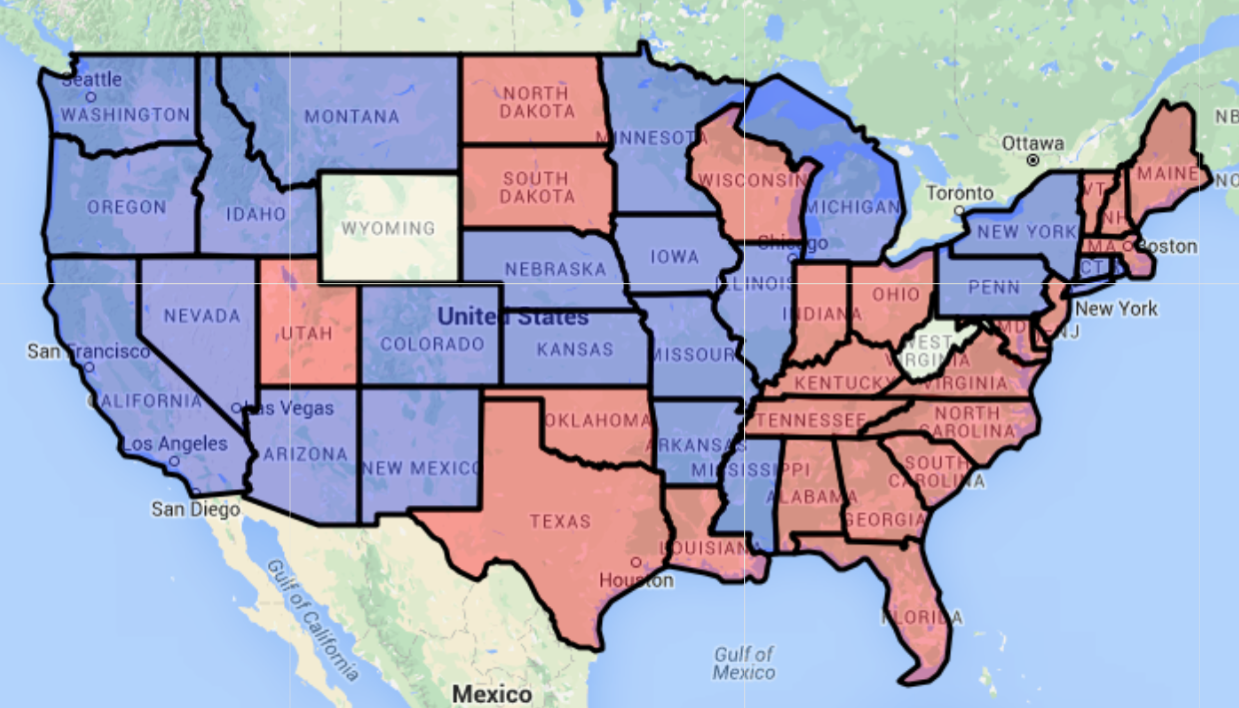
\includegraphics[width=3.5in, height=2.2in]{ContinentalUs.png}
\caption{States won by the candidates - red for Trump and Blue for Clinton.}
\label{ContinentalUs}
\end{figure}

\begin{figure}
\centering
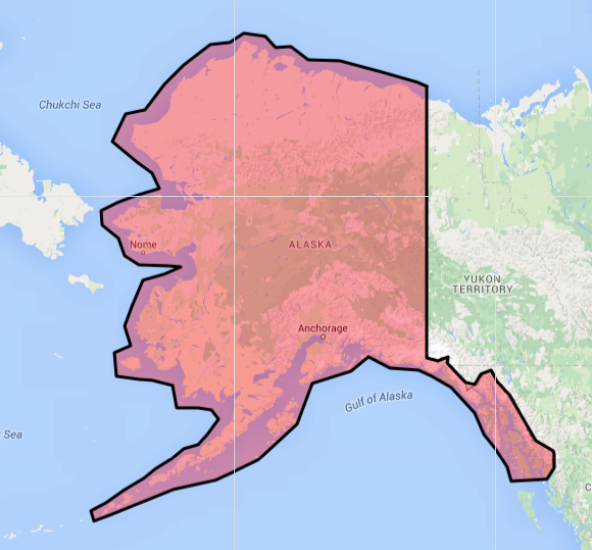
\includegraphics[width=2in, height=2in]{Alaska.png}
\caption{Alaska winner - Trump.}
\label{Alaska}
\end{figure}

\begin{figure}
\centering
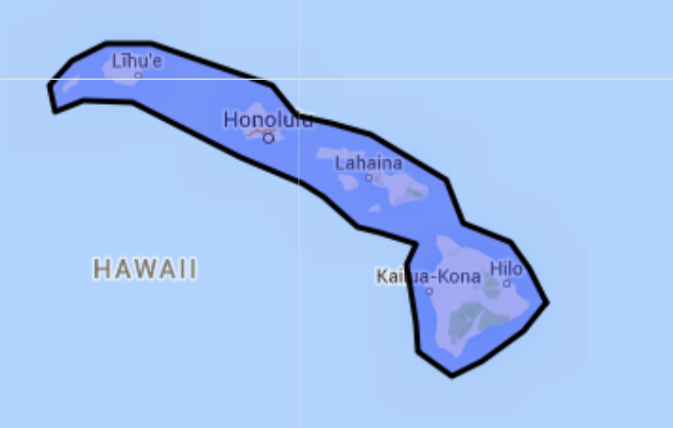
\includegraphics[width=2.5in, height=2.5in]{Hawaii.png}
\caption{Hawaii winner - Clinton.}
\label{Hawaii}
\end{figure}

\subsection{Tweets per day over time}
I did not get tweets that were distributed over the period of study. All the Clinton tweets were for January 29\textsuperscript{th} and 20\textsuperscript{th}, 2016. These were the days I retrieved the tweets and all the tweets retrieved were for those days. All Trump tweets were for January 30\textsuperscript{th} , 31\textsuperscript{st} and February 1\textsuperscript{st} 2016. Due to this reason I do not have data for the trend for tweets per day over time.

\subsection{Number of tweets by time of day}

\begin{figure}
\centering
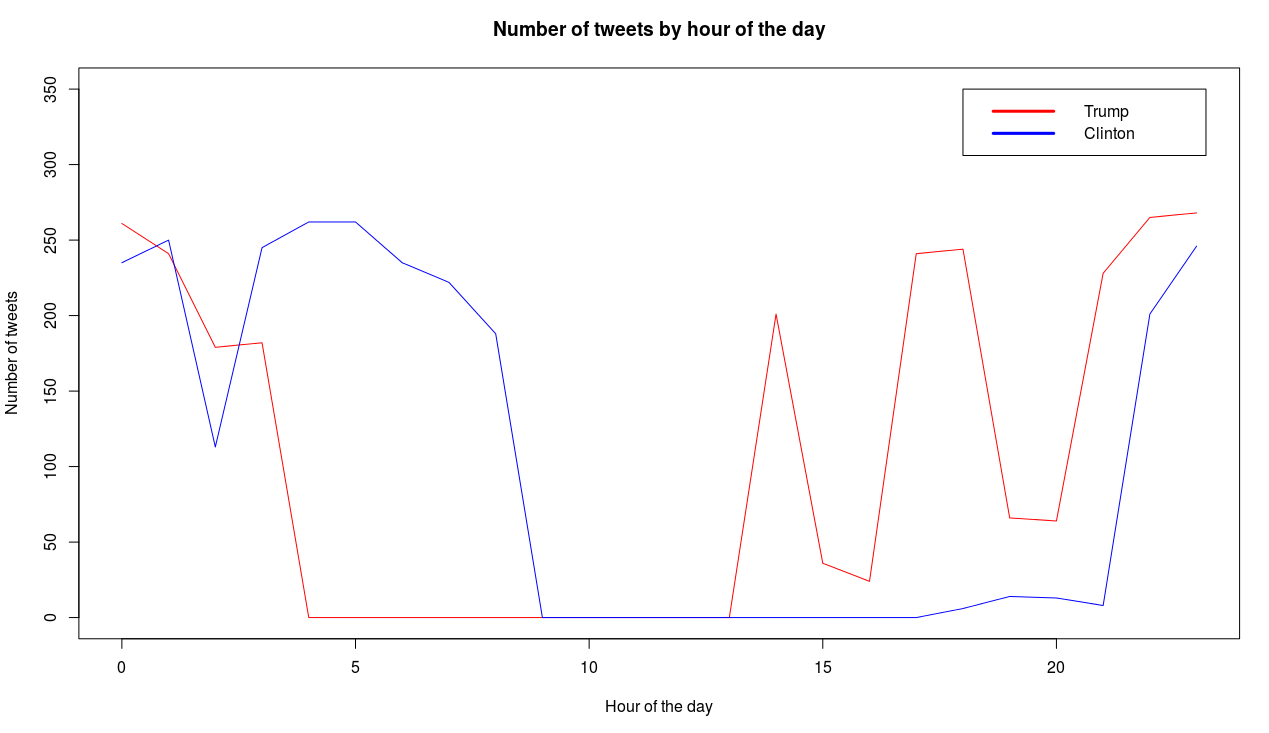
\includegraphics[width=3.5in, height=2.5in]{TweetsByHour.png}
\caption{Number of tweets by time of day.}
\label{TweetTime}
\end{figure}

Figure \ref{TweetTime} shows the number of tweets by time of day. The x-axis shows the hour of the day and the y-axis shows the corresponding number of tweets.\\

It seems that Trump tweeters are intermittently active from 2 pm till 8 pm. After 8 pm, they remain active till around 3 am. Then they are inactive till 2 pm.\\

On the other hand Clinton tweeters are inactive from 9 am till 9 pm and active at other times.\\

Since the tweets that are returned by the Twitter Search API are from around the time the search was run, I have a suspicion that this trend over time of day corresponds to the time the tweets were retrieved. However I am not sure if that is the case or not.
\subsection{Projected Winner}
According to this analysis, the projected winner is Donald Trump with 269 to 264 electoral votes.
%
% The following two commands are all you need in the
% initial runs of your .tex file to
% produce the bibliography for the citations in your paper.
\bibliographystyle{abbrv}
\bibliography{sigproc}  % sigproc.bib is the name of the Bibliography in this case
% You must have a proper ".bib" file
%  and remember to run:
% latex bibtex latex latex
% to resolve all references
%
% ACM needs 'a single self-contained file'!
%
%APPENDICES are optional
%\balancecolumns
\appendix
%Appendix A
\section{Sample Tweets}
\label{sssec:num1} 

\verb user_location: Ohio\\
\verb created_at: Sun Jan 31 17:15:53 +0000 2016\\
\verb id_str: 693845165463752705\\
t\verb ext: RT @samantharonson: Donald Trump has flip-flopped so much that Stephen Colbert hosted a Trump vs. Trump debate https://t.co/Wa8c8WkfTo via ?\\
\verb user_screen_name: christinerod1\\
\verb user_id_str: 27403847\\
\verb place: None\\
\verb user_friends_count: 286\\
\verb user_followers_count: 52\\
\verb user_lang: en\\

\verb user_location: Atlanta, GA\\
\verb created_at: Sun Jan 31 17:25:18 +0000 2016\\
\verb id_str: 693847538554789889\\
\verb text: RT @redsteeze: Also a good modern day analogy of Donald Trump and the Republican Party https://t.co/Gv0L0MimV2\\
\verb user_screen_name: WarDamnGunners\\
\verb user_id_str: 728693384\\
\verb place: None\\
\verb user_friends_count: 533\\
\verb user_followers_count: 463\\
\verb user_lang: en\\

\verb user_location: North Carolina\\
\verb created_at: Mon Feb 01 02:17:10 +0000 2016\\
\verb id_str: 693981384113831936\\
\verb text: RT @SavageNation: BREAKING POLL: Donald Trump Is winning Latino Republicans: Si Se Puede! In new poll on Latino voters finds Don... https:/?\\
\verb user_screen_name: NewsieSc\\
\verb user_id_str: 2946622600\\
\verb place: None\\
\verb user_friends_count: 937\\
\verb user_followers_count: 489\\
\verb user_lang: en\\

\section{Summarized Data}
\label{sssec:num2} 

\begin{figure}
\centering
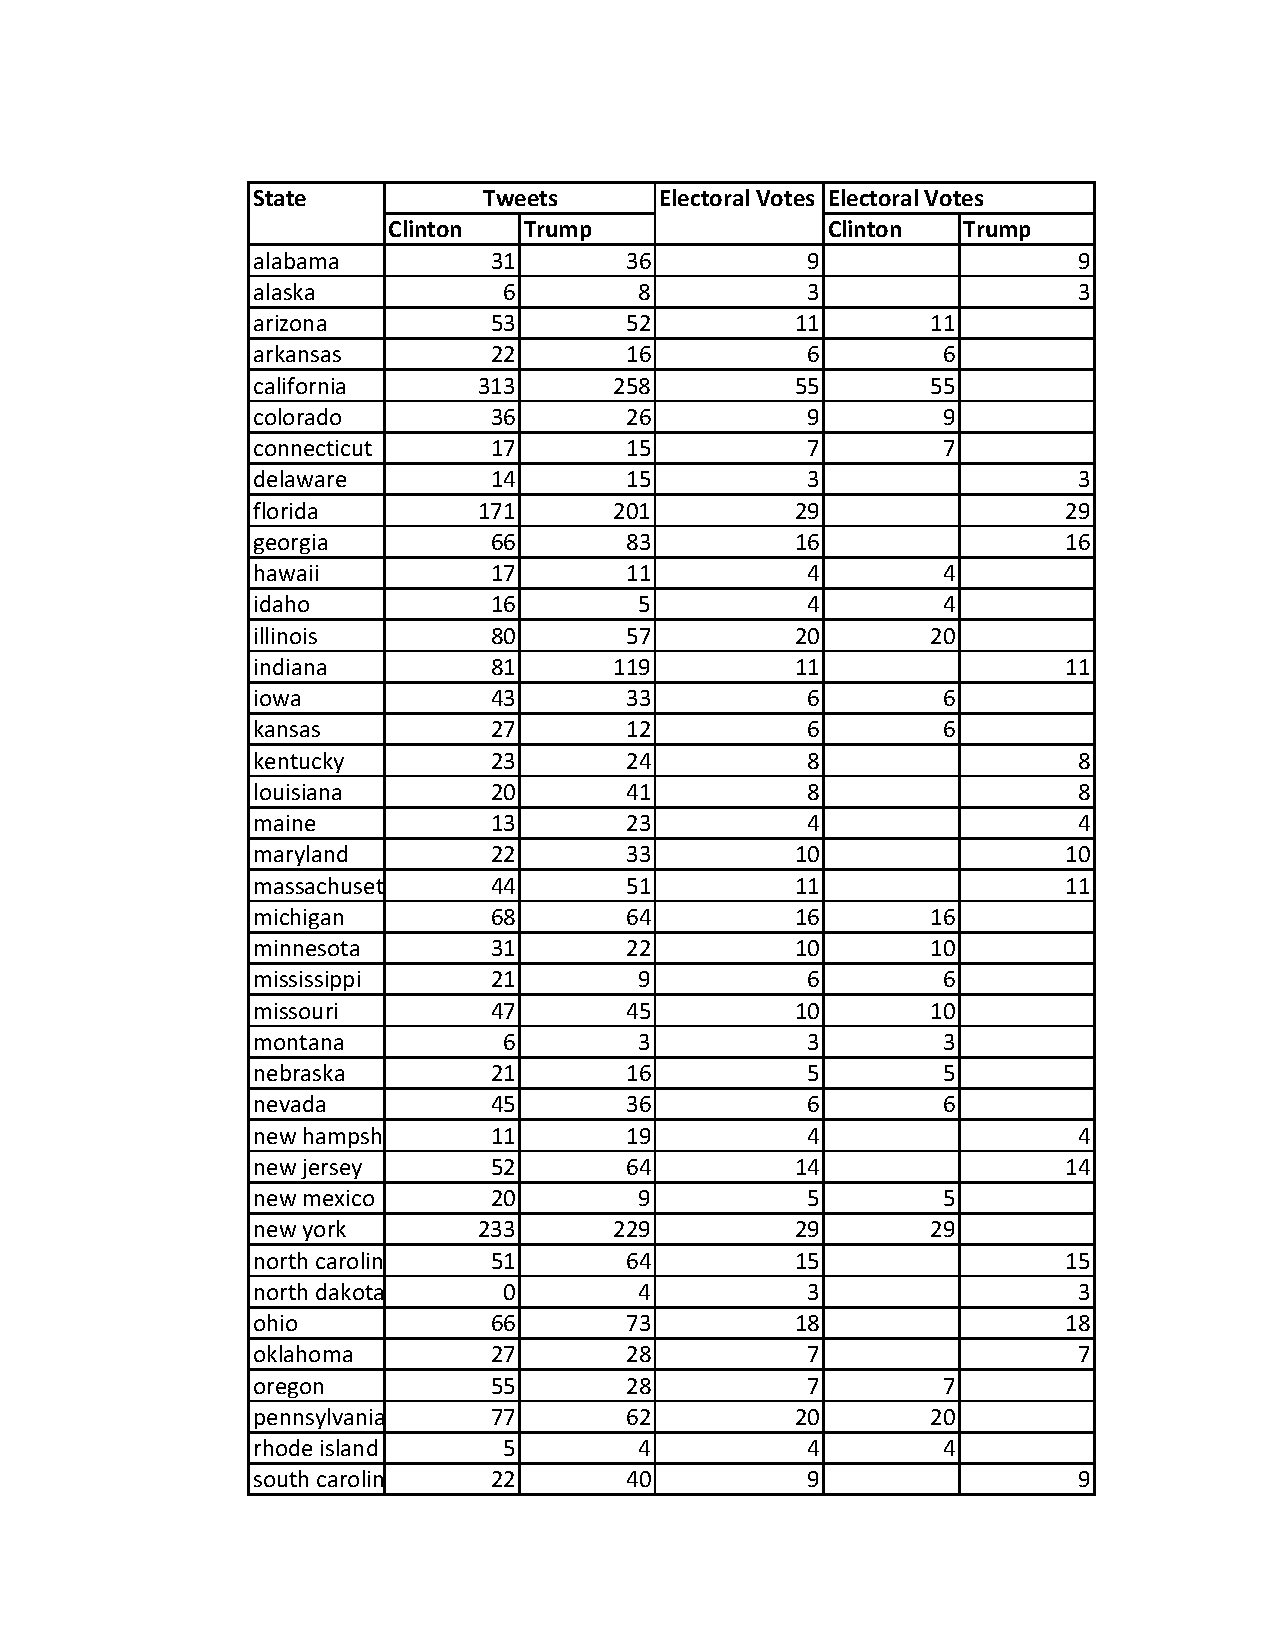
\includegraphics[width=3.5in, height=3.5in]{WinnerCalculation1.pdf}
\caption{Electoral Votes won by state}
\label{WinnerCalculation}
\end{figure}

\begin{figure}
\centering
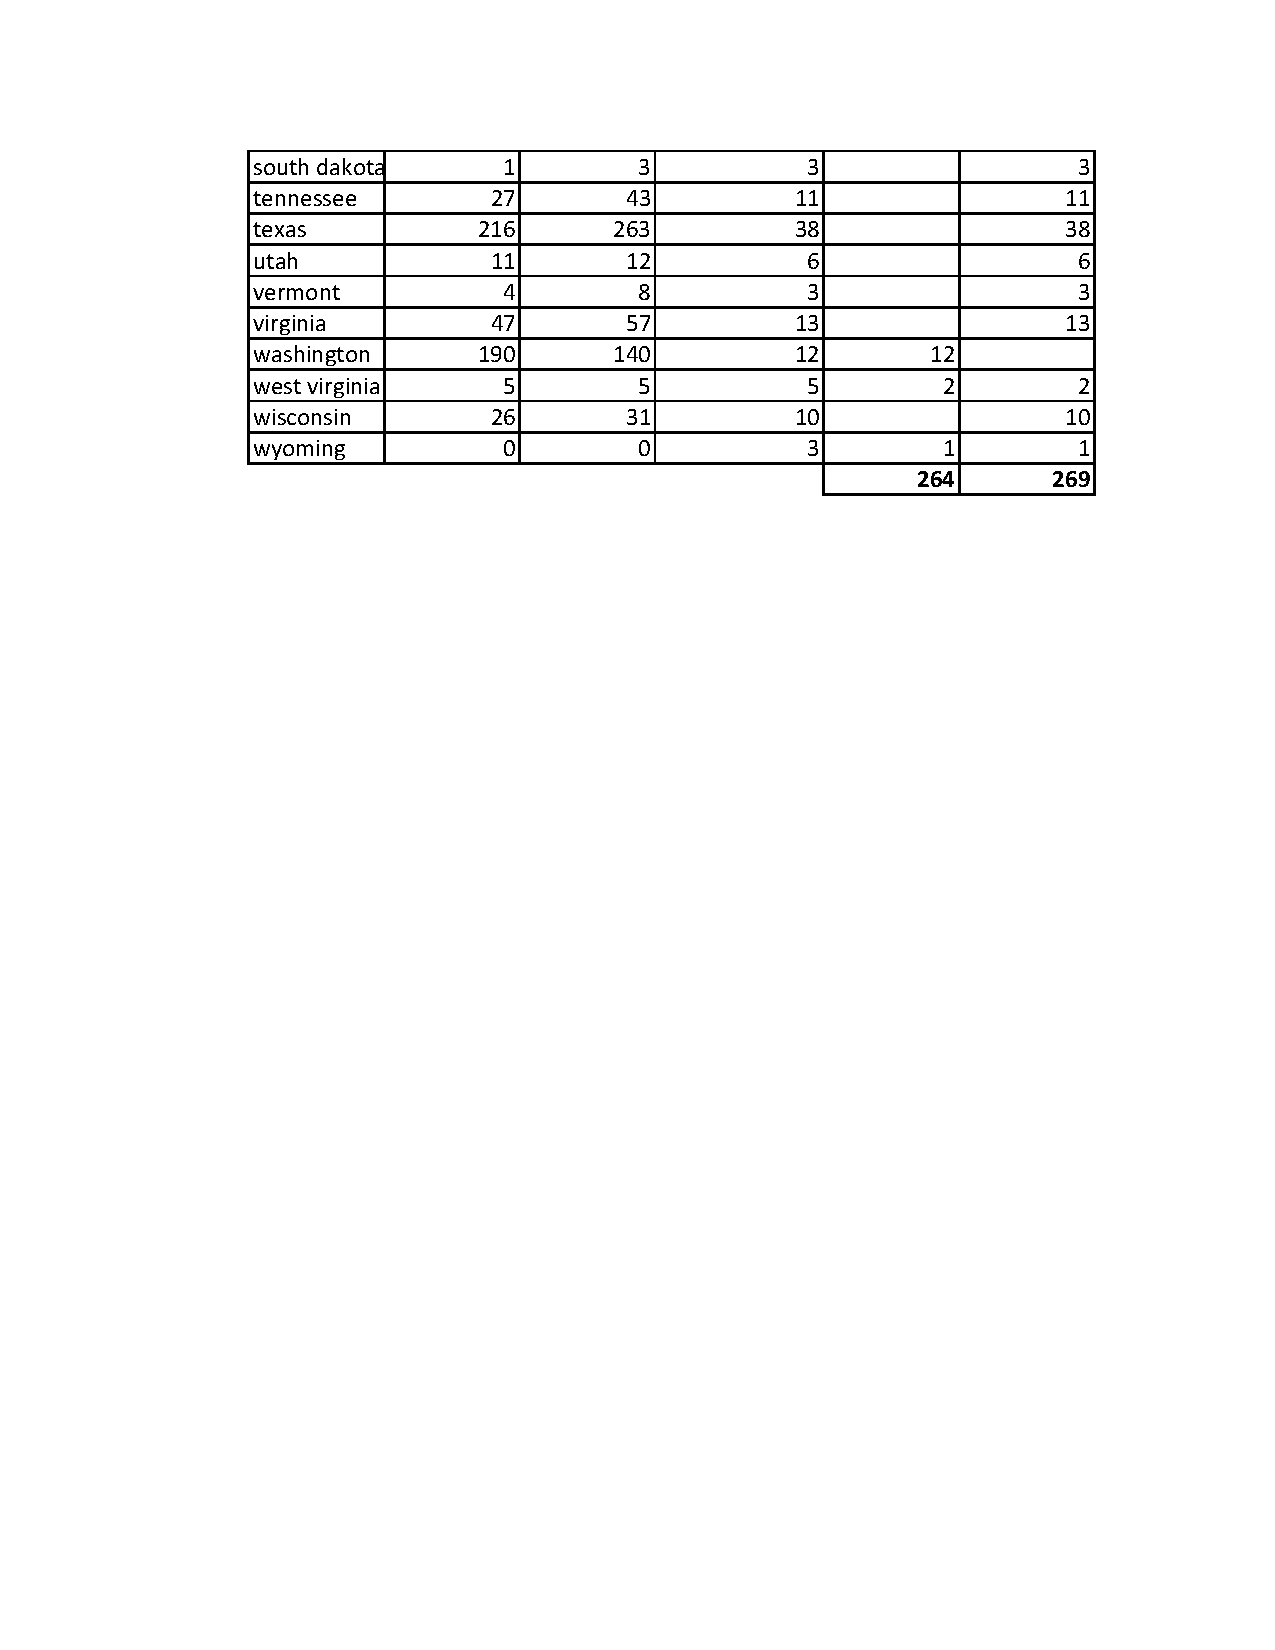
\includegraphics[width=3.5in, height=3.5in]{WinnerCalculation2.pdf}
\caption{Electoral Votes won by state (contd.)}
\label{WinnerCalculation}
\end{figure}
%\balancecolumns % GM June 2007
% That's all folks!
\end{document}
